\documentclass[12pt,table,t]{beamer}

% Packages
\usepackage{xcolor}
\usepackage{eulervm}
\usepackage[norsk]{babel}
\usepackage[utf8]{inputenc}
\usepackage{tabularx}
\usepackage{cancel}


% Theme
\mode<presentation>
{
  \usetheme{Honefoss}
%  \setbeamercovered{transparent}
  \setbeamertemplate{blocks}[rounded]
  \AtBeginPart{\frame[c]{\partpage}}
}

\newcommand{\comment}[1]{{\slshape\color{kvred}#1}}

\title{Where}
\subtitle{-- for bedre referanserammer}
\author{Michael Dähnn, Ingrid Fausk, Geir Arne Hjelle, Ann-Silje
  Kirkvik, Laila Løvhøiden, Eirik Mysen}
\date{Divisjonssamling, 29.\ april 2016}
%\titlegraphic{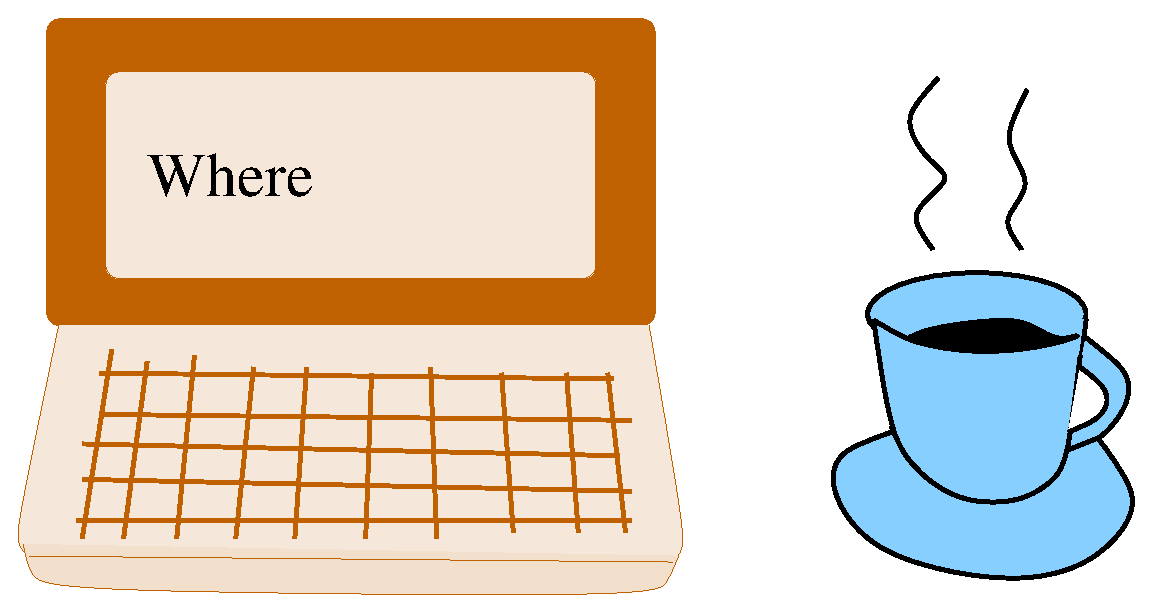
\includegraphics[width=\paperwidth]{figure/where}}

\begin{document}
\frame[plain]{\titlepage}

\begin{frame}{}  % Greit å bare nevne elefanten med en gang ... ?
  \begin{center}
    \vfill {\Huge Where is Geosat?} \\
    \pause
    \vfill {\Huge Where is Geosat!} \\
    \pause
    \hfil \emph{... sånn omtrent ...}
    \vfill
  \end{center}
\end{frame}


\part{Bakgrunn}

\begin{frame}{Where}

  Where er en programvare som vil kunne analysere data fra geodetiske stasjoner som Ny-Ålesund, og gjennom dette
  bidra til utviklingen av bedre globale referanserammer.
  \pause

  \begin{columns}[c]
    \column{0.18\textwidth}
    \begin{center}
      \includegraphics[width=\linewidth]{figure/michael} \\
      Michael
    \end{center}

    \column{0.18\textwidth}
    \begin{center}
      \includegraphics[width=\linewidth]{figure/ingrid} \\
      Ingrid
    \end{center}

    \column{0.18\textwidth}
    \begin{center}
      \includegraphics[width=\linewidth]{figure/geirarne} \\
      Geir Arne
    \end{center}

    \column{0.18\textwidth}
    \begin{center}
      \includegraphics[width=\linewidth]{figure/annsilje} \\
      Ann-Silje
    \end{center}

    \column{0.18\textwidth}
    \begin{center}
      \includegraphics[width=\linewidth]{figure/eirik} \\
      Eirik
    \end{center}
  \end{columns}
\end{frame}


\begin{frame}{Referanserammer}

  Globale referanserammer brukes for å kunne sammenligne posisjoner på forskjellige steder og til forskjellige
  tidspunkt.

  \begin{itemize}
  \item<3-> Referanserammen består av \emph{referansepunkter} man kan måle andre steder mot.
  \item<4-> En utfordring er at man ikke alltid kan måle i en rett linje.
  \item<7-> Ved hjelp av siktelinjer kan man gi hvert punkt en koordinat.
  \item<9-> Koordinatene kan så brukes til å regne ut total avstand.
  \end{itemize}

  \begin{center}
    \includegraphics<2>{figure/referanseramme1a}
    \includegraphics<3>{figure/referanseramme1b}
    \includegraphics<4>{figure/referanseramme2a}
    \includegraphics<5>{figure/referanseramme2b}
    \includegraphics<6>{figure/referanseramme2c}
    \includegraphics<7>{figure/referanseramme2d}
    \includegraphics<8>{figure/referanseramme2e}
    \includegraphics<9>{figure/referanseramme2f}
    \includegraphics<10>{figure/referanseramme2g}
  \end{center}
\end{frame}


\begin{frame}{Referanserammer}

  En utfordring med globale referanserammer er at man velger utgangspunktet (\emph{origo}) i sentrum av jorda.

  \begin{itemize}
  \item<2-> Vi kan ikke måle opp referansepunktene direkte.
  \item<3-> Vi må \emph{gjette} på koordinatene til referansepunktene, og deretter korrigere disse gjennom målinger.
    \begin{itemize}
    \item<3-> Dette kalles å \emph{estimere} posisjonen.
    \end{itemize}
  \item<4-> For best mulige korreksjoner vil vi \emph{kombinere} forskjellige måleteknikker.
  \end{itemize}

  \begin{center}
    \includegraphics<2>{figure/referanseramme4a}
    \includegraphics<3>{figure/referanseramme4b}
    \includegraphics<4>{figure/referanseramme4c}
  \end{center}
\end{frame}


\begin{frame}{Referanserammer}

  Globale referanserammer brukes for å kunne sammenligne posisjoner på forskjellige steder og til forskjellige
  tidspunkt.

  \begin{itemize}
  \item<1-> Ved gjentatte målinger kan man få forskjellig resultat.
  \item<2-> Det kan være mange kilder til usikkerheter.
  \item<3-> Om man antar at referansepunktene flytter på seg \uncover<4->{kan man estimere hastigheter.}
  \end{itemize}

  \begin{center}
    \includegraphics<1>{figure/referanseramme3a}
    \includegraphics<2>{figure/referanseramme3b}
    \includegraphics<3>{figure/referanseramme3c}
    \includegraphics<4>{figure/referanseramme3d}
  \end{center}
\end{frame}


\begin{frame}{Hvorfor gjør vi dette?}
  
  Globale referanserammer er nødvendige for

  \begin{itemize}
  \item å følge utviklingen av klimaet over tid,
  \item å beregne presise satellittbaner, og
  \item utnytte nye muligheter innen stedfesting.
  \end{itemize}
  \pause

  Kartverket ønsker å bidra til utviklingen av bedre globale referanserammer.

  \begin{itemize}
  \item Vi trenger denne kompetansen for å drifte Ny-Ålesund godt.
  \item Den teknologiske utviklingen gjør at geodesien blir stadig mer global.
  \item Global geodesi er bygget opp på \emph{best effort} --- frivillig innsats fra individuelle institusjoner.
  \item 193 land -- alle FN-medlemmene -- har forstått at det er viktig å ivareta og utvikle det globale
    geodesiarbeidet.
  \end{itemize}
\end{frame}


\part{Where-prosjektet}

\begin{frame}{Status primo 2014 (Geosat)}
  Det overordnet viktigste resultatmålet for Geosat-prosjektet:

  \begin{itemize}
  \item Innen utgangen av prosjektet [2.\ juni 2015] må Kartverket ha opparbeidet seg tilstrekkelig kompetanse til å
    utvikle og vedlikeholde programvaren, slik at vi selvstendig kan jobbe videre med å forbedre presisjonen i
    leveransene av baner og referanseramme.\\
    \hfill\emph{BP2 Prosjektplan Geosat}
  \end{itemize}
\end{frame}


\begin{frame}[c]{Geosat -- Kompetanseindikator}
  \footnotesize
  \begin{tabularx}{\textwidth}{Xr|c|c|c|c|c}
    \textbf{Dato} & & \textbf{aug 14} & \textbf{des 14} & \textbf{apr 15} & \textbf{aug 15} & \textbf{mål des} \\
    \hline
    \textbf{VLBI}        & Teori & 0.20 & 0.25 & 0.30 & 0.55 & \emph{0.6} \\
                         & Kode  & 0.10 & 0.15 & 0.30 & 0.40 & \emph{0.6} \\
    \hline
    \textbf{SLR}         & Teori & 0.20 & 0.25 & 0.30 & 0.50 & \emph{0.8} \\
                         & Kode  & 0.15 & 0.20 & 0.30 & 0.50 & \emph{0.8} \\
    \hline
    \textbf{GNSS}        & Teori & 0.20 & 0.20 & 0.30 & 0.35 & \emph{0.7} \\
                         & Kode  & 0.01 & 0.10 & 0.25 & 0.30 & \emph{0.5} \\
    \hline
    \textbf{DORIS}       & Teori & 0.15 & 0.20 & 0.20 & 0.20 & \emph{0.8} \\
                         & Kode  & 0.10 & 0.20 & 0.20 & 0.20 & \emph{0.6} \\
    \hline
    \textbf{Kombinasjon} & Teori & 0.54 & 0.70 & 0.80 & 0.80 & \emph{0.9} \\
                         & Kode  & 0.32 & 0.50 & 0.60 & 0.70 & \emph{0.9} \\
    \hline
    \textbf{Sum}         &       & 1.97 & 2.75 & 3.55 & 4.50 & \emph{7.2} \\
  \end{tabularx}
\end{frame}


\begin{frame}{Sommeren 2015}

  \begin{itemize}
  \item Prosjektgruppa overtok ansvaret for å utvikle og vedlikeholde programvaren Geosat.
  \item En ny arkitektur for programmet ble laget for enklere fremtidig utvikling og vedlikehold. Denne ble senere gitt
    navnet Where.
  \item Enkle modeller for utregning av VLBI-baselinjer og SLR-satellittbaner ble implementert for å teste den nye
    arkitekturen.
  \end{itemize}
\end{frame}


\begin{frame}{Høsten 2015}

  \begin{itemize}
  \item Vi jobbet videre med flytting og nyutvikling av modeller for VLBI og SLR i Where-arkitekturen.
  \item En ny prosjektplan ble utarbeidet, denne gjelder fra 15. oktober 2015.
  \item Vi endret arbeidsmetodikk til smidige prinsipper, med kontinuerlig rapportering av utviklingen i prosjektet.
  \item Ny rapporteringsside: \url{http://nnriap039.statkart.no/where/}
  \item Chalmers / Onsala i Sverige startet en studie av forskjellige programvarer for VLBI-analyse. Vi deltok i denne
    studien.
  \item Per Helge Andersen gikk av med pensjon.
  \end{itemize}
\end{frame}


\begin{frame}{Ny overordnet målsetting for prosjektet}

  {\large\itshape Kartverket skal bidra til utviklingen av bedre globale referanserammer og bli anerkjent for dette
    arbeidet.}
  \vspace*{2ex}
  \pause

  \textbf{Virkemidler}
  \begin{itemize}
  \item Utvikling av verktøy inkludert programvare og metodikk for analyse av romgeodetiske teknikker.
  \item Oppygging av kompetanse.
  \item Deltagelse i fagmiljøer.
  \end{itemize}
\end{frame}


\begin{frame}[c]{Where -- Prosjektindikator}
  \footnotesize
  \begin{tabularx}{\textwidth}{Xr|r|r|r|r}
    \textbf{Dato} & & \textbf{des 15} & \textbf{apr 16} & \textbf{aug 16} & \textbf{mål des} \\
    \hline
    \textbf{VLBI}  & Modeller (15)           &  17\% & 100\% &       & \emph{100\%} \\
                   & Rammeverk (5)           &  50\% &  72\% &       & \emph{100\%} \\
    \hline
    \textbf{SLR}   & Modeller (20)           &  45\% &  90\% &       & \emph{100\%} \\
                   & Rammeverk (6)           &  33\% &  58\% &       & \emph{100\%} \\
    \hline
    \textbf{GNSS}  & Modeller (30)           &   0\% &  10\% &       &  \emph{40\%} \\
                   & Rammeverk (6)           &   0\% &  20\% &       &  \emph{60\%} \\
    \hline
    \textbf{DORIS} & Modeller \phantom{(20)} &   0\% &   0\% &       &   \emph{0\%} \\
                   & Rammeverk (6)           &   0\% &   0\% &       &  \emph{20\%} \\
    \hline
    \textbf{Annet} & Kompetanse (17)         &   0\% &  59\% &       & \emph{100\%} \\
                   & Anerkjennelse (3)       &   0\% &  67\% &       & \emph{100\%} \\
    \hline
    \textbf{Sum}   &                         & 1.45\phantom{\%} & 4.76\phantom{\%} &
                                                   \phantom{\%} & \emph{7.2\phantom{\%}} \\
  \end{tabularx}
\end{frame}


\part{Where-programvaren}

\begin{frame}{Where -- Arkitektur}

  \begin{center}
    \includegraphics<1>[width=\textwidth]{figure/code_structure}
    \includegraphics<2>[width=\textwidth]{figure/code_structure_current}
  \end{center}
\end{frame}


%%% Kombinasjon
\section{Kombinasjon av teknikker}

\begin{frame}[c]{}
  \begin{center}
    {\Huge Kombinasjon av teknikker}
  \end{center}
\end{frame}


\begin{frame}{Hvordan beregnes globale referanserammer?}

  \begin{itemize}
  \item En stasjonsposisjon, $XYZ$ -- kan ikke måles med meterstokk.
  \item Gjetter på hva $XYZ$ skal være: $(XYZ)_0$.
  \item Klokker + modell for virkeligheten gir ny $XYZ$.
  \item Denne oppdaterte posisjonen $XYZ$ er avhengig av gjetningen $(XYZ)_0$!
  \end{itemize}
  \pause

  Vilkårlighet i $XYZ$ gir vilkårlighet i referanseramme:
  \begin{itemize}
  \item Transformasjoner
  \end{itemize}
\end{frame}


\begin{frame}{Estimering av stasjonsposisjoner}

   \begin{itemize}
    \item Where ser $XYZ$ fra forskjellige vinkler/ståsteder ved å samkjøre informasjonen fra forskjellige datatyper:
      \begin{itemize}
      \item VLBI, SLR, GNSS, DORIS
      \end{itemize}
    \item Dette reduserer vilkårligheten.
    \item Posisjonen $XYZ$ blir bestemt av data og ikke gjetning.
   \end{itemize}
\end{frame}


\begin{frame}{Prinsipper for kombinasjonen}

  \begin{itemize}
   \item Data + modell gir $XYZ$ (\emph{estimering})
   \item Gir også usikkerheten i $XYZ$ 
   \item Usikkerheten er upålitelig, men må være riktig for å kombinere informasjonen
   \item Nye vektingsstrategier
   \item Ikke ekskludere måter å kombinere informasjon på
   \end{itemize}
\end{frame}


\begin{frame}{Styrker ved teknikkene}

  I kombinasjonen bidrar hver teknikk med sine styrker:

  \begin{description}
  \item[SLR] Jordsentrum, lengden av en meter
  \item[GNSS] Tett nettverk, mye data, jordrotasjon
  \item[VLBI] Kobling mot verdensrommet, lengden av en meter, jordrotasjon
  \item[DORIS] Jevnt fordelt nettverk, presise satellittbaner
  \end{description}
\end{frame}


%%% SLR
\section{SLR - Satellite Laser Ranging}

\begin{frame}[c]{}
  \begin{center}
    {\Huge SLR -- Satellite Laser Ranging}
  \end{center}
\end{frame}


\begin{frame}{SLR -- Satellite Laser Ranging}

  \begin{center}
    \includegraphics[width=0.4\textwidth]{figure/lageos1}
  \end{center}
\end{frame}


\begin{frame}{Satellittene er utstyrt med reflektorer}  

  \begin{center}
    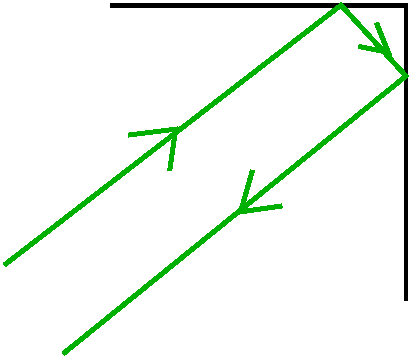
\includegraphics[width=0.6\textwidth]{figure/laser}
  \end{center}
\end{frame}


\begin{frame}{SLR-stasjon og -satellitt}

  \begin{center}
    \includegraphics[width=0.6\textwidth]{figure/SLR}
  \end{center}
\end{frame}


\begin{frame}{Status for utviklingen av SLR-koden}

  \begin{itemize}
  \item Har implementert modeller for krefter som virker på satellitten.  
  \item Modeller fra IERS Conventions og fra forskjellige forskningsartikler.
  \item Modellene inngår i likningene som vi løser for å beregne en bane for en uke for Lageos. 
  \item Kan gjenbrukes for andre satellitter og andre teknikker. 
  \end{itemize}
\end{frame}


\begin{frame}{Hva påvirker satellittbaner}

  \begin{center}
    \includegraphics[width=0.8\textwidth]{figure/sat.jpg}
  \end{center}
\end{frame}


\begin{frame}{Hva påvirker hvordan vi oppfatter satellittbanene}
  \begin{itemize}
  \item Forsinkelser gjennom troposfæren.
  \item Stasjonen flytter også på seg grunnet tidejordskrefter og ocean loading-effekter.
  \item Laserstrålen reflekteres ikke i massesenteret til satellitten.
    \begin{itemize}
    \item<2-> Satellitten er ikke egentlig en rund ball.
    \item<2-> Ikke alle fotonene treffer den samme reflektoren.
    \end{itemize}
  \end{itemize}

  \begin{center}
    \includegraphics<2->[width=0.3\textwidth]{figure/corners}
  \end{center}
\end{frame}


\begin{frame}{Pulsen er ikke like fin når den kommer tilbake}
  \begin{center}
    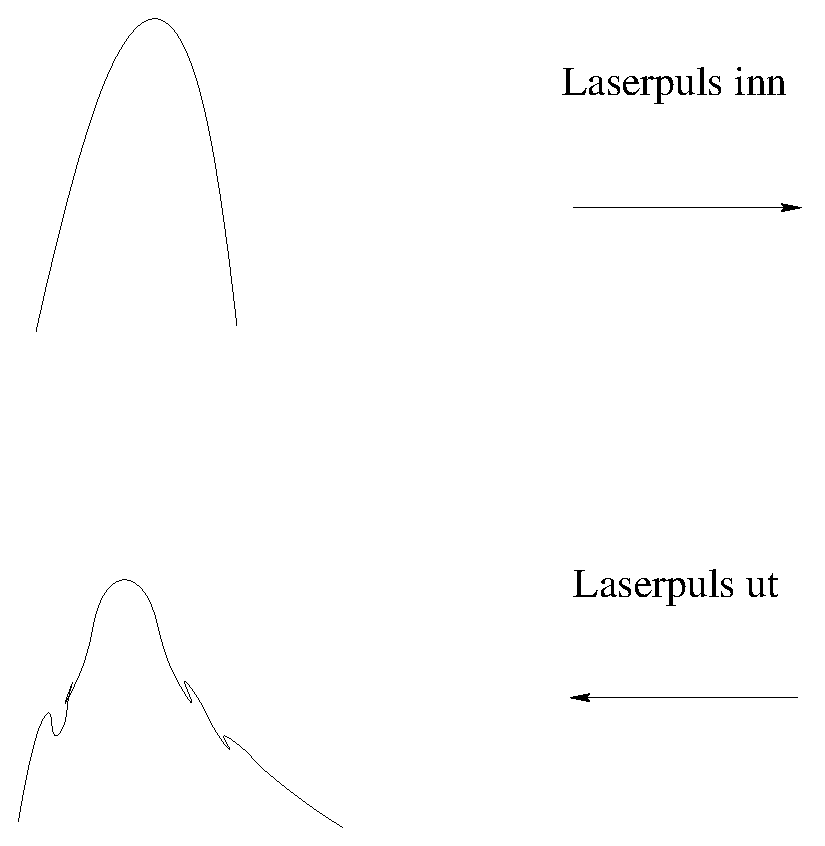
\includegraphics[width=0.6\textwidth]{figure/pulse}
  \end{center}
\end{frame}


\begin{frame}{Videre arbeid med SLR}

  \begin{itemize}
  \item Videre testing av de ulike modellene.
  \item Kjøretiden må drastisk ned.
  \item Legge inn empiriske krefter og estimere range bias.
  \item Når satellittbanen er god vil vi estimere stasjonsposisjoner.
  \end{itemize}
\end{frame}


%%% GNSS
\section{GNSS - Global Navigation Satellite System}

\begin{frame}[c]{}
  \begin{center}
    {\Huge GNSS -- Global Navigation Satellite System}
  \end{center}
\end{frame}


\begin{frame}{GNSS -- Global Navigation Satellite System}
  \includegraphics<1>[width=\textwidth]{figure/multi_gnss_overview}
  \includegraphics<2>[width=\textwidth]{figure/multi_gnss_selection}

  \vfill

  \begin{itemize}
  \item<2> Samarbeid med GNSS monitoreringsprosjektet
  \end{itemize}
\end{frame}


\begin{frame}{GNSS -- Posisjoneringsprinsippet}
  \includegraphics<1>[width=\textwidth]{figure/gnss_how_it_works_1}
  \includegraphics<2>[width=\textwidth]{figure/gnss_how_it_works_2}
  \includegraphics<3>[width=\textwidth]{figure/gnss_how_it_works_3}
  \includegraphics<4>[width=\textwidth]{figure/gnss_how_it_works_4}
  \includegraphics<5>[width=\textwidth]{figure/gnss_how_it_works_5}
  \includegraphics<6>[width=\textwidth]{figure/gnss_how_it_works_6}
  \includegraphics<7>[width=\textwidth]{figure/gnss_how_it_works_7}
  \includegraphics<8>[width=\textwidth]{figure/gnss_how_it_works_8}
  \includegraphics<9>[width=\textwidth]{figure/gnss_how_it_works_9}
  \includegraphics<10>[width=\textwidth]{figure/gnss_how_it_works_10}
  \includegraphics<11>[width=\textwidth]{figure/gnss_how_it_works_11}
\end{frame}


\begin{frame}{GNSS -- Dataflyt}
  \includegraphics<2>[width=0.7\textwidth]{figure/gnss_workflow_1}
  \includegraphics<3>[width=0.7\textwidth]{figure/gnss_workflow_2}
  \includegraphics<4>[width=0.7\textwidth]{figure/gnss_workflow_3}
  \includegraphics<5>[width=0.7\textwidth]{figure/gnss_workflow_4}
  \includegraphics<6>[width=0.7\textwidth]{figure/gnss_workflow_5}
  \includegraphics<7>[width=0.7\textwidth]{figure/gnss_workflow_6}
\end{frame}


\begin{frame}{Precise Point Positioning (PPP)}
  \includegraphics<1>[width=0.7\textwidth]{figure/gnss_workflow_7}
  \includegraphics<2>[width=0.7\textwidth]{figure/gnss_workflow_8}
\end{frame}


\begin{frame}{GNSS-status i Where}
  \vspace*{-0.5cm}
  \includegraphics<2>[width=0.7\textwidth]{figure/gnss_workflow_status_1}
  \includegraphics<3>[width=0.7\textwidth]{figure/gnss_workflow_status_2}
  \includegraphics<4>[width=1.0\textwidth]{figure/gnss_status_residuals}
\end{frame}


\begin{frame}{Videre arbeid med GNSS}
  \begin{itemize}
  \item Først fokusere på GPS og Galileo.
  \item Implementere Precise Point Positioning (PPP)-løsning.
  \item Se på dataediteringsrutinene til Oddgeir.
  \item Kompetanseutvikling (bl.a. dokumentasjon av Geosat-koden).
  \end{itemize}
\end{frame}


%%% VLBI
\section{VLBI - Very Long Baseline Interferometry}

\begin{frame}[c]{}
  \begin{center}
    {\Huge VLBI -- Very Long Baseline Interferometry}
  \end{center}
\end{frame}


\begin{frame}{VLBI -- Observasjon}
  \begin{center}
    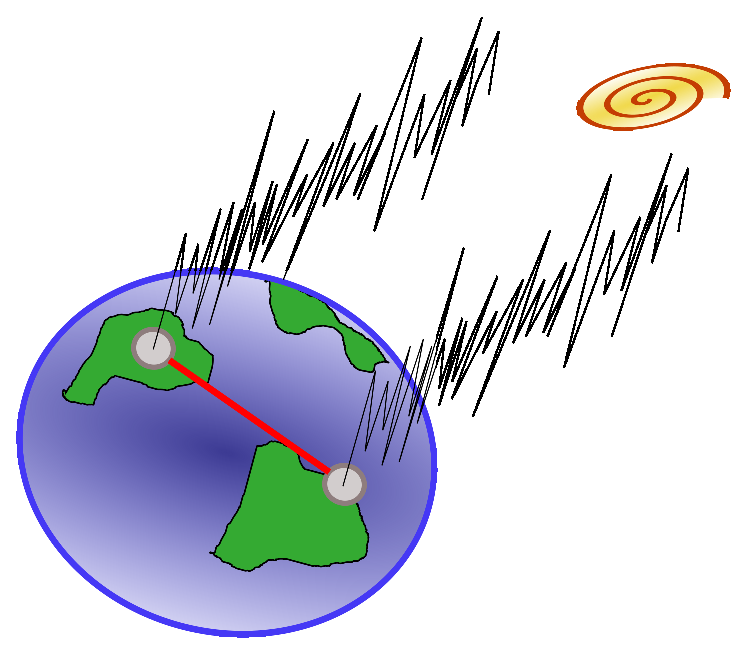
\includegraphics[width=0.6\textwidth]{figure/vlbi_concept}
  \end{center}
\end{frame}


\begin{frame}{VLBI -- Modell og residual}
  \Large
  \begin{block}{Teoretisk forsinkelse}
    \vspace*{-0.7cm}
    \begin{align*}
      \tau &= \tau_{geometric} + \tau_{grav} + \tau_{tropo} + \tau_{axisoffset} \\
           &+ \tau_{thermdef} + \tau_{clock} + \tau_{cable} + \tau_{iono}
    \end{align*}
  \end{block}

  \begin{block}{Residual}
    \begin{center}
      $residual = observasjon - modell$
    \end{center}
  \end{block}
\end{frame}


\begin{frame}{VLBI Analysis Software Comparison Campaign}

  \begin{itemize}
  \item Utføres av Grzegorz Klopotek (Ph.D-student) ved Chalmers University of Techonology.
  \item Vi har valgt å delta med programvaren Geosat fordi Where ikke var påbegynt når forespørselen kom.
  \item Det har vært en veldig nyttig og lærerik øvelse for kritisk gjennomgang av kildekoden.
  \end{itemize}
\end{frame}


\begin{frame}{VLBI Analysis Software Comparison Campaign}

  {\itshape ``The main goal of the VASCC 2015 is to compare different VLBI analysis software packages on the basis of
    computed theoretical delay.''}

  \begin{itemize}
  \item $residual = \xcancel{observasjon} - modell$
  \item $\tau = \tau _{geometric} + \tau _{grav} + \tau _{tropo} + \tau _{axisoffset}$ \\
    $\phantom{\tau\, } + \tau _{thermdef} + \xcancel{\tau _{clock}} + \xcancel{\tau _{cable}} + \xcancel{\tau _{iono}}$
  \end{itemize}
\end{frame}


\begin{frame}[fragile,c]{VASCC -- Deltakere}
  \footnotesize
  \newcolumntype{R}[1]{>{\hsize=#1\hsize\raggedright\arraybackslash}X}
  \begin{tabularx}{\textwidth}{|R{0.55}|R{1.45}|}
    \hline
    \rowcolor{kvblue}\color{white}\textbf{Programvare} & \color{white}\textbf{Institusjon} \\
    \hline
    \textbf{Bernese GNSS} & Technische Universität München  \\
    \hline
    \textbf{c5++} & Chalmers University of Technology \\
    \hline
    \textbf{Calc11} & Goddard Space Flight Center, NASA \\ 
    \hline
    \textbf{Calc11}, \textbf{SCORR} & Shanghai Astronomical Observatory , Chinese Academy of Sciences \\
    \hline
    \textbf{DOGS-RI}, \textbf{OCCAM} & Technische Universität  München,  Deutsches Geodätisches Forschungsinstitut \\
    \hline
    \textbf{Geosat} & Norwegian Mapping Authority  \\
    \hline
    \textbf{GINS} & Laboratoire d'Astrophysique de Bordeaux  \\
    \hline
    \textbf{GLORIA}, \textbf{Calc11} & Paris Observatory  \\
    \hline 
    \textbf{ivg::ASCOT} & University of Bonn \\
    \hline
    \textbf{OCCAM} & Geoscience Australia \\
    \hline
    \textbf{VieVS} & University of Tasmania \\
    \hline
  \end{tabularx}
\end{frame}


\begin{frame}{VASCC -- Foreløpige resultater}
  \begin{itemize}
  \item Under en millimeter (RMS) samsvar mellom 6 programvarer så langt (Calc11(GSFC), DOGS-RI, c5++, ivg::ASCOT,
    SCORR, VieVS).
  \item Bugs og feiltolkninger av konvensjoner er oppdaget i flere av programvarene (inkludert Geosat).
  \item Arbeidet pågår fremdeles.
  \item Kan brukes som en benchmark for å teste modellene i Where.
  \end{itemize}
\end{frame}


\begin{frame}{Videre arbeid med VLBI}

  \begin{itemize}
  \item Nytt format for observasjonsdata er i ferd med å bli tatt i bruk.
  \item Utregning av partieltderiverte.
  \item Estimering av stasjonskoordinater, jordrotasjonsparametere, troposfære og klokker.
  \item Skrive resultater til SINEX og andre etablerte filformater.
  \end{itemize}
\end{frame}


\section{Demo av programvaren}

\begin{frame}[c]{}
  \begin{center}
    {\Huge Where -- Live Demo}
  \end{center}
\end{frame}

\begin{frame}{Where -- Live Demo}

  \begin{itemize}
  \item Kjøring av VLBI med bare konsensusmodellen.
  \item Ser at forskjellige modeller kjøres.
  \item Se på resultater i There.
  \item Gjør ny kjøring med alle modeller.
  \item Sammenlign resultater i There, forbedrede residualer.
  \item Oppdag et klokkebrudd.
  \item Fiks et klokkebrudd, se forbedring i There.
  \end{itemize}
\end{frame}

\end{document}
